%!TEX root = ../paper.tex

\begin{figure}
	\centering
	\begin{subfigure}{0.23\textwidth}
		\centering
		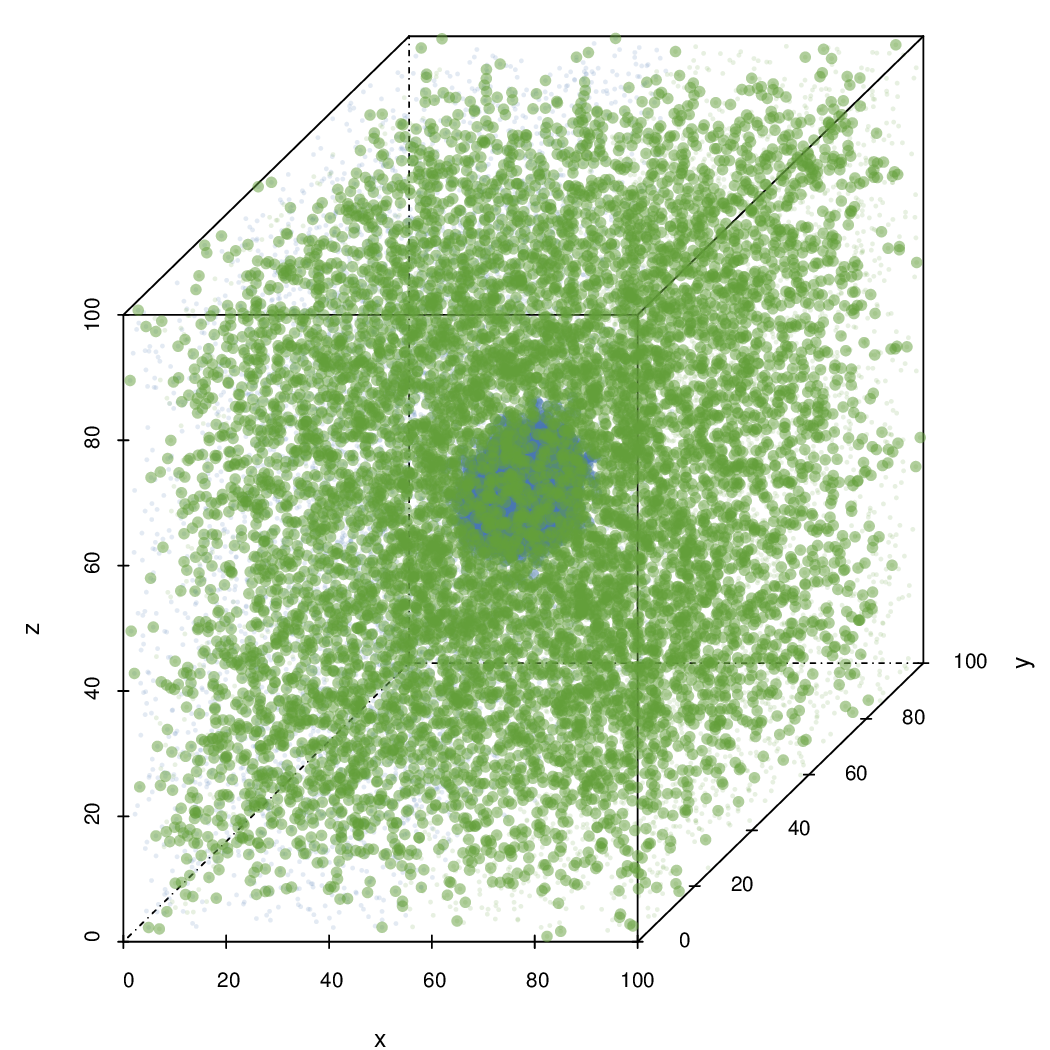
\includegraphics[keepaspectratio=true, width=\textwidth, height=0.23\textheight]{discussion/img/ferdosi_1_abs_error_mbeSmallerThansambe.pdf}
		\caption{Dataset \ferdosiOne}
		\label{fig:discussion:singleSphere:mbeLowerError:ferdosi1}
	\end{subfigure}
	\begin{subfigure}{0.23\textwidth}
		\centering
		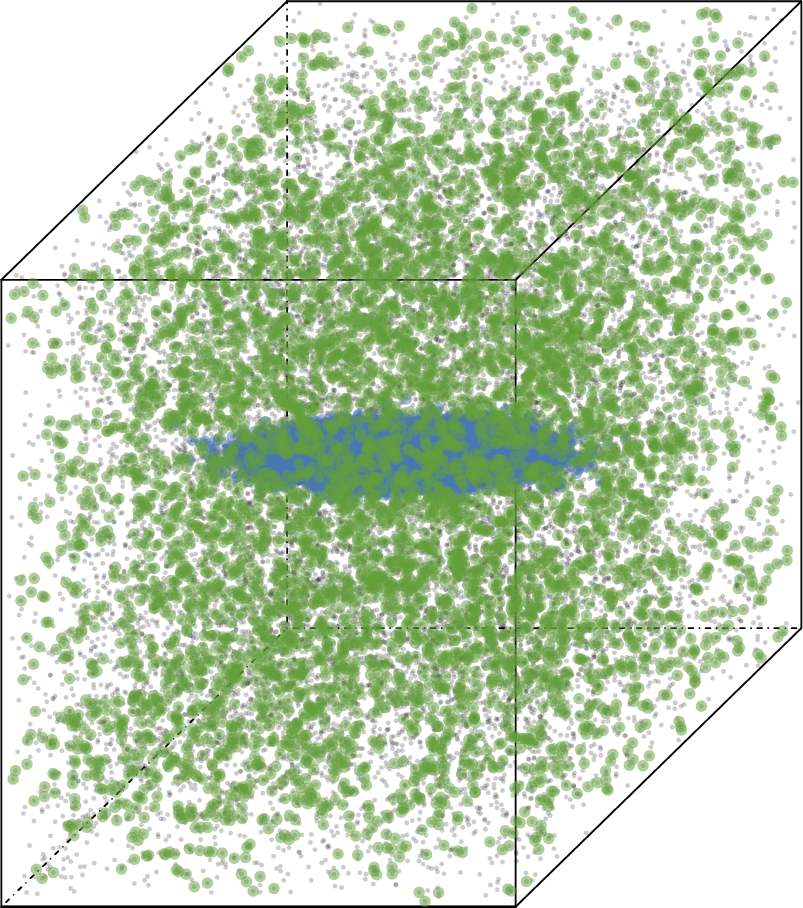
\includegraphics[keepaspectratio=true, width=\textwidth, height=0.23\textheight]{discussion/img/baakman_1_abs_error_mbeSmallerThansambe.pdf}
		\caption{Dataset \baakmanOne}
		\label{fig:discussion:singleSphere:mbeLowerError:baakman1}
	\end{subfigure}	
	\begin{subfigure}{0.23\textwidth}
		\centering
		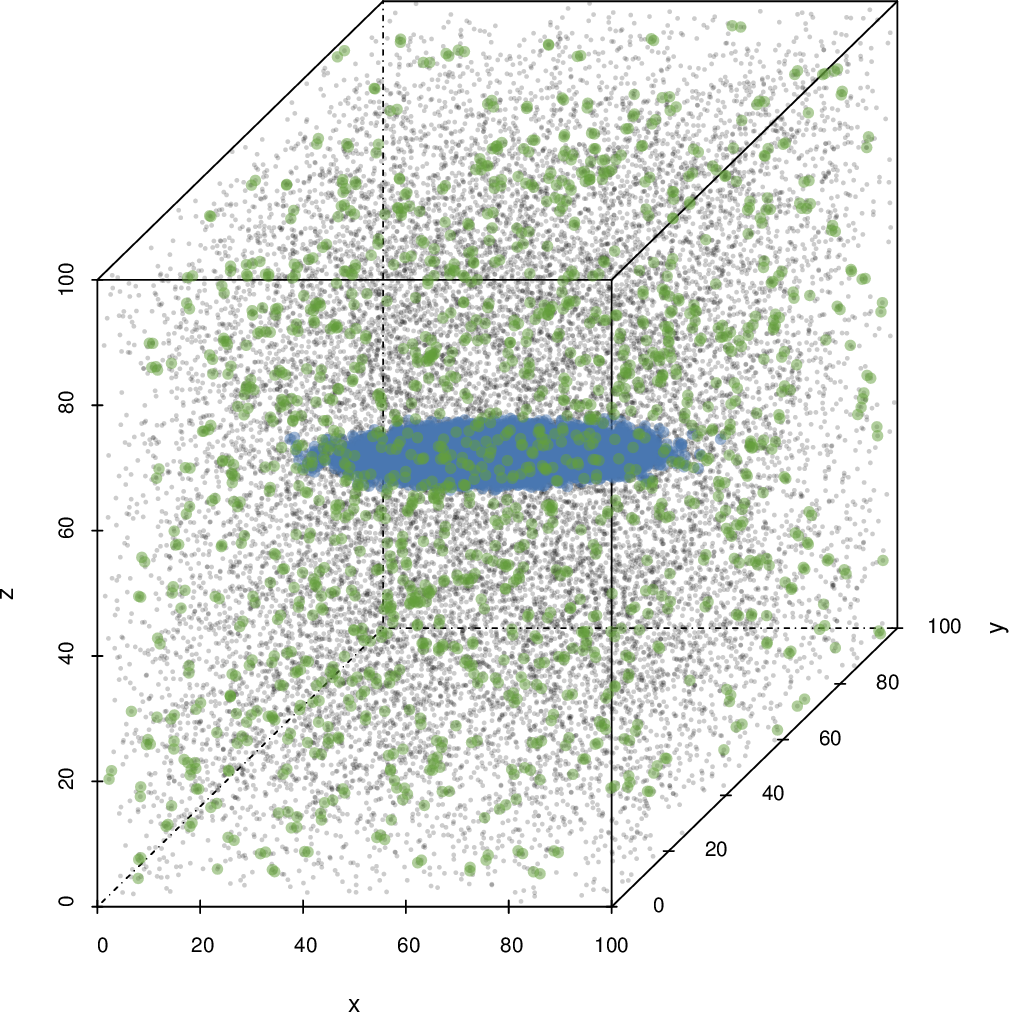
\includegraphics[keepaspectratio=true, width=\textwidth, height=0.23\textheight]{discussion/img/baakman_4_abs_error_mbeSmallerThansambe.pdf}
		\caption{Dataset \baakmanFour}
		\label{fig:discussion:singleSphere:mbeLowerError:baakman4}
	\end{subfigure}		
	\begin{subfigure}{0.23\textwidth}
		\centering
		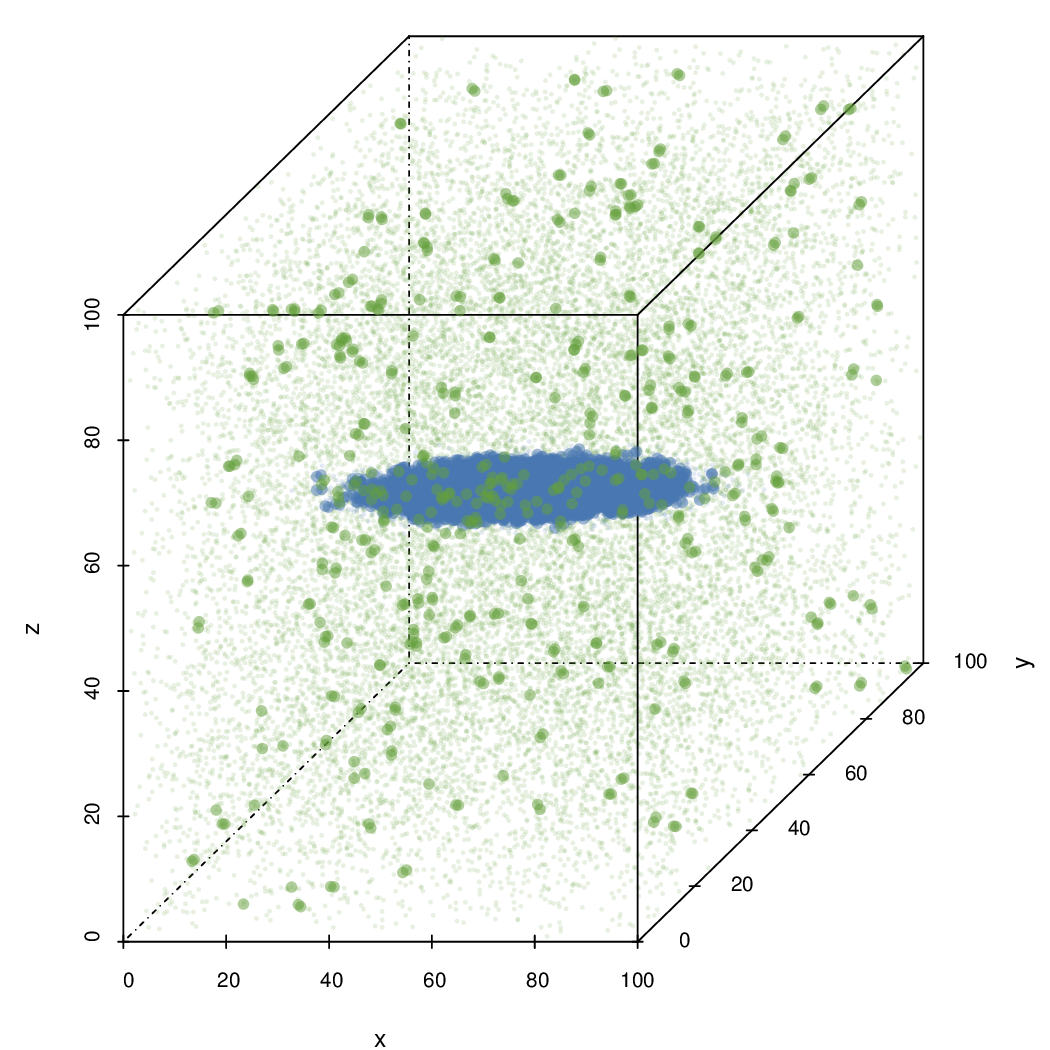
\includegraphics[keepaspectratio=true, width=\textwidth, height=0.23\textheight]{discussion/img/baakman_5_abs_error_mbeSmallerThansambe.pdf}
		\caption{Dataset \baakmanFive}
		\label{fig:discussion:singleSphere:mbeLowerError:baakman5}
	\end{subfigure}			
	\caption{Low opacity scatter plot of dataset %
		\subref{fig:discussion:singleSphere:mbeLowerError:ferdosi1} \ferdosiOne, %
		\subref{fig:discussion:singleSphere:mbeLowerError:baakman1} \baakmanOne, %
		\subref{fig:discussion:singleSphere:mbeLowerError:baakman4} \baakmanFour, and%
		\subref{fig:discussion:singleSphere:mbeLowerError:baakman5} \baakmanFive, %
		with an overlay of larger points with a higher opacity where the absolute error of \sambe is larger than or equal to the absolute error of \mbe.}
	\label{fig:discussion:singleSphere:mbeLowerError}
\end{figure}

% Introduction
The scatter plots of the datasets with a single Gaussian in \cref{fig:discussion:singleSphere:mbeLowerError} emphasize the points where the absolute error of the symmetric estimator is smaller than that of the shape-adaptive estimator. 

	% Ferdosi 1
		% ALl POINTS
		% SAMBE better than MBE: 2.828800000000000e+04 (4.727588742563005e+01 percent)
		% MBE better than SAMBE: 3.154800000000000e+04 (5.272411257436994e+01 percent)
		% MBE equal to SAMBE: 0.000000000000000e+00 (0.000000000000000e+00 percent)
		
		% Component 0
		% MSE(MBE, SAMBE):
		%  1.245351981191544e-08	& 1.335673957702697e-08

		% SAMBE better than MBE: 1.773700000000000e+04 (4.434250000000000e+01 percent)
		% MBE better than SAMBE: 2.226300000000000e+04 (5.565750000000001e+01 percent)
		% MBE equal to SAMBE: 0.000000000000000e+00 (0.000000000000000e+00 percent)

		% Component 1
		% MSE(MBE, SAMBE):
		%  1.046361645486837e-11	& 1.282383835662826e-11

		% SAMBE better than MBE: 1.055100000000000e+04 (5.319116757410768e+01 percent)
		% MBE better than SAMBE: 9.285000000000000e+03 (4.680883242589232e+01 percent)
		% MBE equal to SAMBE: 0.000000000000000e+00 (0.000000000000000e+00 percent)	


		% The overlay plot
		\Cref{fig:discussion:singleSphere:mbeLowerError:ferdosi1} shows that the shape-adaptive estimator results outperforms the symmetric estimators on most points near the boundary of the dataset. It also seems to illustrate that that \mbe results in a lower error than \sambe on the other points, however the raw data shows that on \num{5.272411257436994e+01}\% of the full dataset, and on \num{5.565750000000001e+01} \% of the Gaussian component the symmetric estimator results in a lower absolute error.
		% The shape of the kernels
		Reviewing the shape of the kernels used for the points in dataset \ferdosiOne we find that the used kernels are all near spherical. The kernels with the largest differences between their eigenvalues are associated with points near the boundary of the dataset. 
		% Largest differnces in estimated values between kernels. 
		The largest differences in error between the two estimators can be found near the center of the Gaussian component, where the shape-adaptive kernels are relatively spherical. The difference between the two estimators at these points is caused by the number of points used to estimate the density, for most of these points \sambe uses too many points which results in an overestimated density. 

	% Baakman 1
		% Component -1
		% MSE(MBE, SAMBE):
		%  1.494313211797496e-08	& 1.544094229246398e-08
		% SAMBE better than MBE: 2.509400000000000e+04 (4.193796376763152e+01 percent)
		% MBE better than SAMBE: 2.680000000000000e+04 (4.478909017982485e+01 percent)
		% MBE equal to SAMBE: 7.942000000000000e+03 (1.327294605254362e+01 percent)

		% Component 0
		% MSE(MBE, SAMBE):
		%  2.231981590358483e-08	& 2.306388047782812e-08
		% SAMBE better than MBE: 1.924800000000000e+04 (4.812000000000000e+01 percent)
		% MBE better than SAMBE: 2.061300000000000e+04 (5.153250000000001e+01 percent)
		% MBE equal to SAMBE: 1.390000000000000e+02 (3.475000000000000e-01 percent)

		% Component 1
		% MSE(MBE, SAMBE):
		%  6.778671444628963e-11	& 6.901612718035766e-11
		% SAMBE better than MBE: 5.846000000000000e+03 (2.947166767493447e+01 percent)
		% MBE better than SAMBE: 6.187000000000000e+03 (3.119076426698931e+01 percent)
		% MBE equal to SAMBE: 7.803000000000000e+03 (3.933756805807623e+01 percent)

		% Overlay plot
		The results in \cref{fig:discussion:singleSphere:mbeLowerError:baakman1} are comparable to those in \cref{fig:experiment:singlesphere:ferdosi1}, however there seem to be fewer points of the noise component where the absolute error of using the symmetric-kernel is lower than using a shape-adaptive kernel. Reviewing the raw data shows that this difference is primarily caused by the \num{7.803000000000000e+03} points for which both estimators estimate the same density. Due to the elongated shape of the distribution its shape influences the kernel of fewer shapes of the noise component resulting in more spherical kernels, which results in the same density estimate for a larger number of points. 
		% The shape of the kernels
		As in dataset \ferdosiOne the points with the most ellipsoidal kernels are positioned near the boundaries of the dataset, where \sambe outperforms \mbe. 
		% Largest differences in estiamted values between estimators
		The points whose differences in estimated densities are largest are, as in dataset \ferdosiOne, found near the mean of the Gaussian distribution. At first this seems counterintuitive since the kernels are relatively spherical near the Gaussian component, however we expect that due to the high density of points in that area a small change to the shape of the kernel has a large effect. This is confirmed by the large differences in the number of patterns that are used in the density estimate of the points near the mean of the Gaussian component between the two estimators. 

	%Baakman 4
	% Component -1
	% MSE(MBE, SAMBE):
	%  2.945143538188240e-08	& 2.971553835946330e-08

	% SAMBE better than MBE: 2.061700000000000e+04 (3.445584597900929e+01 percent)
	% MBE better than SAMBE: 2.132900000000000e+04 (3.564576509124942e+01 percent)
	% MBE equal to SAMBE: 1.789000000000000e+04 (2.989838892974129e+01 percent)	
	% Component 0
	% MSE(MBE, SAMBE):
	%  4.404296246131644e-08	& 4.443607459199309e-08

	% SAMBE better than MBE: 1.926500000000000e+04 (4.816250000000000e+01 percent)
	% MBE better than SAMBE: 1.988200000000000e+04 (4.970500000000000e+01 percent)
	% MBE equal to SAMBE: 8.530000000000000e+02 (2.132500000000000e+00 percent)


	% Component 1
	% MSE(MBE, SAMBE):
	%  2.710168671393879e-11	& 3.105311540244085e-11

	% SAMBE better than MBE: 1.352000000000000e+03 (6.815890300463804e+00 percent)
	% MBE better than SAMBE: 1.447000000000000e+03 (7.294817503528937e+00 percent)
	% MBE equal to SAMBE: 1.703700000000000e+04 (8.588929219600726e+01 percent)	
	
	% Overlay Plot
	In \cref{fig:discussion:singleSphere:mbeLowerError:baakman4} we observe that the \mbe outperforms \sambe on very few points in dataset \baakmanFour, to be exact on \num{92.7051824965} percent of the points the absolute error of the shape-adaptive estimator was at least as low as the error of the symmetric estimator. Once again we attribute this difference in performance to the elongated shape of the Gaussian component. 
	% Shape of the kernels
	Reviewing the shape of the kernel we find kernels with a strongly adapted shape both near the boundary of the dataset, where \sambe outperforms \mbe, and near the Gaussian component.
	% Largest differences in estimated values between estimators
	Near the mean of this component we also find the biggest differences in estimated densities between the two estimators. 

	%Baakman 5
	
	\todo[inline]{Wat zien we in het plotje?}
	\todo[inline]{Iets over de vorm van de kernels.}
	\todo[inline]{What is the influence of the distance to the mean?}

% General observations 
\todo[inline]{Waarom sambe zoveel beter op randen, zo veel slechter in de buurt van de mean van de distributie? Seems to be a general problem, not a single sphere problem.}
\todo[inline]{Near the mean: very little shape adaption, but large difference in estimated densites: strong effect of small change due to high density of points?}
\todo[inline]{Near the boundaries: a lot of shape adaption: relatively small differences in estimated densites: effect not a astrong due to lower density of the points. }



\oldStuff

%General Discussion
	%Small difference between two estimators
		% Confirm with plots
		The most striking observation of \cref{s:results:singleGaussian} is the small difference between the densities approximated by the two estimators. To investigate what caused these differences, we first verified if the differences in \mse were caused by a select group of points, to that end we compared the density estimations of the individual points by plotting the results of \sambe as a function of \mbe. These plots do not indicate a specific group of points that causes the difference in \MSE between the two estimators within datasets.
		
		% Investigate the points with the largest differences
		Investigating the points that result in the biggest difference in estimated density between estimators we find that in the datasets with a single Gaussian they all lie near the mean of the Gaussian distribution. Furthermore the density of these points are both over and underestimated by the shape-adaptive estimator, if the first is the case generally fewer points have contributed to the \mbe density than to the \sambe density. If the shape-adaptive estimator underestimates densities it generally uses far less points to base its approximation on than the symmetric estimator uses for that same point. This suggest that some of the kernels near the mean of the Gaussian our to big, allowing a contribution to some points that they should not contribute to, and conversely that some are too small. 

		% Investigate the kernels.
		Reviewing the shape of the kernels used by the shape-adaptive estimator we find some differences between the datasets. 
			% Ferdosi 1
			In dataset \ferdosiOne, as expected due to the spherical Gaussian, the three eigenvalues of the kernels hardly differ, indicating that the kernels are near spherical. 
			% Baakman 1
			In the elongated version of this dataset, a couple of points have ellipsoidal kernels, as indicated by the eigenvalues of their covariance matrices. Since all these points are positioned in corners of the dataset we contribute the shape of these kernels to their position, instead of to any influence from the Gaussian distribution. This problem could possibly be solved by taking a larger neighborhood into account when determining the kernel shape. 
			% Baakman 4
			In dataset \baakmanFour numerous points have strongly ellipsoidal kernels, a lot of these points can be found at the boundaries of the datasets. However a lot of these point are also placed in and around the Gaussian distribution. 
			% Baakman 5
			The same holds for dataset \baakmanFive.
		%Some general blaat
		\todo[inline]{This is wrong! SAMBE works better at the boundaries for multisphere sets, quite likely also the case for single sphere.}	
		There is no way for the kernel determination algorithm to distinguish between points that lie at the edge of a dataset, or a point that lies at the boundary of the distribution. If the density of interest lies in large area of irrelevant points one could discard the estimated densities at the boundaries, since these suffer from this boundary-effect.
			
